\documentclass[10pt,a4paper]{report}

% --- Essential Packages ---
\usepackage[utf8]{inputenc}
\usepackage[T1]{fontenc}
\usepackage[margin=0.65in,top=0.65in,bottom=0.65in]{geometry}
\usepackage{times}
\usepackage{amsmath,amssymb,amsfonts}
\usepackage{graphicx}
\usepackage{booktabs}
\usepackage{tabularx}
\usepackage{multirow}
\usepackage{caption}
\usepackage{subcaption}
\usepackage{algorithm}
\usepackage{algpseudocode}
\usepackage{listings}
\usepackage{microtype}
\usepackage{cite}
\usepackage{xcolor}
\usepackage{fancyhdr}
\usepackage{titlesec}
\usepackage{etoolbox}
\usepackage[colorlinks=true, linkcolor=blue!80!black, citecolor=blue!80!black, urlcolor=blue!80!black]{hyperref}

% --- Float & Layout Tuning ---
\renewcommand{\topfraction}{0.95}
\renewcommand{\bottomfraction}{0.85}
\renewcommand{\textfraction}{0.05}
\renewcommand{\floatpagefraction}{0.85}
\setlength{\parskip}{2pt}
\setlength{\parindent}{12pt}
\setcounter{tocdepth}{1}
\setcounter{secnumdepth}{2}

% --- Continuous Flow for College Report ---
\makeatletter
\patchcmd{\chapter}{\if@openright\cleardoublepage\else\clearpage\fi}{}{}{}
\patchcmd{\chapter}{\clearpage}{}{}{}
\makeatother

% --- Colors ---
\definecolor{primary}{RGB}{18, 52, 86}
\definecolor{secondary}{RGB}{30, 144, 255}
\definecolor{codegray}{rgb}{0.5,0.5,0.5}
\definecolor{backcolour}{rgb}{0.96,0.96,0.96}

% --- Listings Formatting ---
\lstdefinestyle{mystyle}{
    backgroundcolor=\color{backcolour},   
    commentstyle=\color{codegray},
    keywordstyle=\color{primary}\bfseries,
    numberstyle=\tiny\color{codegray},
    stringstyle=\color{red!70!black},
    basicstyle=\ttfamily\scriptsize,
    breaklines=true,                 
    captionpos=b,                    
    numbers=left,                    
    numbersep=4pt,                  
    tabsize=2,
    frame=single
}
\lstset{style=mystyle}

% --- Header & Footer ---
\pagestyle{fancy}
\fancyhf{}
\setlength{\headheight}{12pt}
\fancyhead[L]{\footnotesize\color{primary}\textbf{Machine Learning Project Report}}
\fancyhead[R]{\footnotesize\nouppercase{\leftmark}}
\fancyfoot[C]{\footnotesize\thepage}
\renewcommand{\headrulewidth}{0.4pt}
\renewcommand{\footrulewidth}{0.4pt}

% --- Compact Chapter & Section Styling ---
\titleformat{\chapter}[hang]
  {\normalfont\bfseries\color{primary}\large}
  {\thechapter.\ }
  {0.3em}
  {\large}
  [\vspace{0.2ex}\titlerule]

\titleformat{name=\chapter,numberless}[hang]
  {\normalfont\bfseries\color{primary}\large}
  {}
  {0pt}
  {\large}
  [\vspace{0.2ex}\titlerule]

\titlespacing*{\chapter}{0pt}{8pt}{6pt}
\titlespacing*{\section}{0pt}{6pt}{3pt}
\titlespacing*{\subsection}{0pt}{4pt}{2pt}

\begin{document}

% ==============================================================================
% PAGE 1: COLLEGE PROJECT TITLE PAGE
% ==============================================================================
\begin{titlepage}
    \centering
    \vspace*{0.2cm}
    {\normalsize\textbf{A MACHINE LEARNING PROJECT REPORT ON}\par}
    \vspace{0.4cm}
    {\Large\bfseries\color{primary} BINARY PERSON SEGMENTATION USING FULLY CONVOLUTIONAL U-NET ARCHITECTURE WITH HYBRID OBJECTIVE OPTIMIZATION\par}
    \vspace{0.25cm}
    {\small\textit{An Empirical Investigation on the Penn-Fudan Pedestrian Dataset Across Augmentation, Learning Rate Tuning, Loss Formulations, and Model Capacity Scaling}\par}
    
    \vspace{0.6cm}
    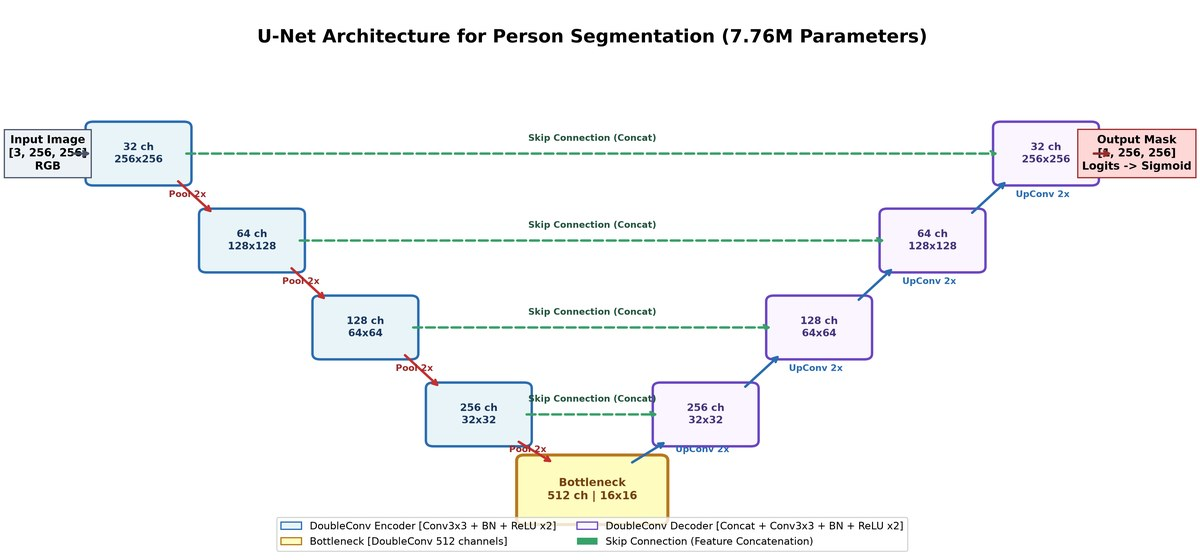
\includegraphics[width=0.24\linewidth]{figures/unet_architecture.jpg}\par
    \vspace{0.6cm}
    
    {\small\textbf{Submitted in partial fulfillment of the requirements for the award of the degree of}\par}
    \vspace{0.15cm}
    {\large\textbf{\color{primary}BACHELOR OF TECHNOLOGY}\par}
    {\small\textbf{in}\par}
    {\large\textbf{COMPUTER SCIENCE AND ENGINEERING}\par}
    
    \vspace{0.6cm}
    \begin{minipage}[t]{0.45\textwidth}
        \begin{flushleft} \small
            \textbf{Submitted by:}\\
            \textbf{Mohith Chandra}\\
            \textit{Roll No: CS-2022-XXXX}\\
            Department of CSE
        \end{flushleft}
    \end{minipage}
    \hfill
    \begin{minipage}[t]{0.45\textwidth}
        \begin{flushright} \small
            \textbf{Under the Guidance of:}\\
            \textbf{Project Supervisor / Guide}\\
            Assistant Professor\\
            Department of CSE
        \end{flushright}
    \end{minipage}
    
    \vfill
    {\small\textbf{DEPARTMENT OF COMPUTER SCIENCE AND ENGINEERING}\par}
    {\normalsize\textbf{INSTITUTE OF TECHNOLOGY}\par}
    {\footnotesize Academic Year 2026--2027\par}
    \vspace{0.2cm}
\end{titlepage}

% ==============================================================================
% PAGE 2: ABSTRACT & TOC (PRELIMINARY PAGES)
% ==============================================================================
\pagenumbering{roman}
\setcounter{page}{2}

\chapter*{Abstract}
\addcontentsline{toc}{chapter}{Abstract}
Pixel-level pedestrian segmentation represents a foundational capability in modern computer vision systems, underpinning safety-critical applications in autonomous driving, mobile robotics, urban video surveillance, and intelligent transportation infrastructure. However, high-fidelity segmentation in real-world urban scenes is challenged by variable human poses, occlusions, scale diversity, background clutter, and severe class imbalance between foreground pedestrians ($23.2\%$) and ambient scene elements ($76.8\%$). In this college project, we design, implement, and evaluate an end-to-end deep learning framework for binary person segmentation trained from scratch on the Penn-Fudan Pedestrian Dataset ($170$ urban images, $345$ pedestrian instances). We formulate an optimized four-stage Fully Convolutional U-Net architecture comprising an encoder-decoder backbone with long-range skip connections, batch normalization, and channel-preserving transposed convolutions ($7.76$M parameters). To address class imbalance and optimize both pixel-level entropy and boundary overlap, we formulate a composite objective function combining Binary Cross-Entropy (BCE) with logits and smooth Dice Loss.

Through an extensive multi-phase empirical investigation across ten systematic experimental stages, we evaluate the impact of synchronized geometric data augmentation (horizontal flip with probability $p=0.5$ and multi-scale zoom within $[0.9, 1.1]$), learning rate optimization ($\eta \in \{10^{-3}, 5\times 10^{-4}, 10^{-4}\}$), loss weight balancing ($\alpha \cdot \mathcal{L}_{\text{BCE}} + \beta \cdot \mathcal{L}_{\text{Dice}}$), and architectural capacity scaling ($16$, $32$, and $48$ base filters). Controlled validation on an untouched $25$-image validation set demonstrates that our optimized configuration ($32$ base channels, learning rate $\eta = 5 \times 10^{-4}$, $\alpha = 1.5, \beta = 0.5$) achieves a peak validation Intersection-over-Union (IoU) of $\mathbf{0.7739}$ and F1-score of $\mathbf{0.8725}$, representing a $+3.92\%$ relative IoU improvement over the non-augmented baseline ($0.7447$). When evaluated on the held-out test split of $27$ previously unseen urban images, the model demonstrates robust generalization with a global pixel IoU of $\mathbf{0.7483}$, global F1-score of $\mathbf{0.8560}$, global recall of $\mathbf{0.8936}$, and a mean per-image IoU of $\mathbf{0.7616} \pm \mathbf{0.1339}$ (median $0.7664$). Qualitative and quantitative error analysis reveals that performance bottlenecks stem primarily from unannotated background pedestrians and severe object occlusion rather than architectural inadequacy. All code, data splits, and checkpoints are fully reproducible.

\vspace{0.4em}
\noindent\textbf{Keywords:} Semantic Segmentation, Deep Learning, U-Net Architecture, Penn-Fudan Pedestrian Dataset, Dice Loss, Binary Cross-Entropy, Computer Vision.

\vspace{0.8cm}
\tableofcontents
\vspace{0.4cm}
\listoffigures
\vspace{0.4cm}
\listoftables
\newpage

% ==============================================================================
% MAIN REPORT
% ==============================================================================
\pagenumbering{arabic}
\setcounter{page}{1}

% ------------------------------------------------------------------------------
% CHAPTER 1: INTRODUCTION
% ------------------------------------------------------------------------------
\chapter{Introduction}
\label{chap:introduction}

\section{Background and Motivation}
Pedestrian detection and segmentation constitute core perceptual tasks in modern artificial intelligence and computer vision. With the rapid deployment of autonomous navigation systems, advanced driver assistance systems (ADAS), unmanned aerial vehicles, and urban video analytics, computer vision systems must reliably delineate human subjects at pixel-level granularity under arbitrary physical conditions. Unlike coarse bounding box detection, which provides only spatial localization via rectangular coordinates, semantic segmentation yields precise object boundaries. This structural precision is crucial in scenarios where spatial margins are minimal, such as an autonomous vehicle navigating near a sidewalk or an automated service robot maneuvering in crowded indoor environments.

The challenge of segmenting pedestrians in unstructured urban scenes originates from high inter-class and intra-class variability. Human subjects exhibit non-rigid deformations, diverse poses (walking, sitting, running, turning), variable clothing textures, varying aspect ratios, and frequent partial or complete occlusions by urban infrastructure, street furniture, bicycles, and fellow pedestrians. Furthermore, illumination fluctuations, low-contrast shadows, complex background textures (such as brick facades, street signage, and vehicular reflections), and significant scale disparities between foreground pedestrians and distant figures exacerbate the segmentation complexity. 

The Penn-Fudan Pedestrian Dataset \cite{wang2007pennfudan} has emerged as an authoritative benchmark for evaluating pedestrian perception models. It comprises high-resolution images of urban pedestrians captured from campus and urban environments with verified pixel-level ground-truth segmentations. While modern deep architectures trained on massive web-scale datasets (such as MS COCO or Cityscapes) demonstrate impressive transferability, developing robust, sample-efficient, from-scratch deep segmentation models on constrained data distributions remains a critical open problem in academic research and edge-device deployments. This research investigates the full lifecycle of training an optimized Fully Convolutional U-Net \cite{ronneberger2015unet} from scratch on the Penn-Fudan dataset, methodically optimizing training dynamics, data augmentation, loss formulations, and architectural capacity.

\section{Problem Statement}
Given an arbitrary RGB natural scene image $\mathbf{X} \in \mathbb{R}^{H \times W \times 3}$, binary person segmentation seeks to compute a dense binary mask $\mathbf{Y} \in \{0, 1\}^{H \times W}$ such that:
\begin{equation}
\mathbf{Y}_{i,j} = 
\begin{cases}
1, & \text{if pixel } (i,j) \text{ belongs to a human pedestrian}, \\
0, & \text{otherwise (background, vehicle, infrastructure, or clutter)}.
\end{cases}
\end{equation}

In practical training scenarios on the Penn-Fudan dataset, this task poses several mathematical and structural challenges:
\begin{enumerate}
    \item \textbf{Severe Spatial Scale Variation:} Foreground pedestrians range from close-up subjects occupying over $40\%$ of the image area to distant pedestrians occupying less than $2\%$ of total pixels. A fixed receptive field cannot simultaneously capture fine limb boundaries and broad torso semantics.
    \item \textbf{Class Imbalance:} In urban scenes, background pixels overwhelmingly outnumber pedestrian pixels ($76.8\%$ background vs. $23.2\%$ pedestrian). Standard Binary Cross-Entropy loss is dominated by easy background negatives, leading to sub-optimal boundary delineation.
    \item \textbf{High-Frequency Spatial Detail Loss:} Successive spatial pooling operations in standard convolutional backbones degrade spatial resolution, blurring thin limbs, walking canes, and overlapping pedestrian silhouettes.
    \item \textbf{Data Scarcity and Overfitting:} With only 170 annotated images available, deep convolutional networks with millions of parameters risk severe empirical overfitting unless regularized through controlled data augmentations, structural bottlenecks, and validated optimization schedules.
\end{enumerate}

\section{Objectives}
The overarching objective of this project is to develop, train, optimize, and thoroughly analyze an end-to-end deep learning framework for binary pedestrian segmentation from scratch, without reliance on pre-trained backbones:
\begin{enumerate}
    \item Construct a leak-free, deterministic data pipeline that transforms raw variable-resolution images and multi-instance pedestrian masks into standardized $256 \times 256$ binary segmentation pairs.
    \item Formulate and implement a custom U-Net architecture from first principles using PyTorch, incorporating double-convolution blocks, batch normalization, channel-preserving transposed up-convolutions, and long-range skip connections.
    \item Implement a numerically stable hybrid loss function combining Binary Cross-Entropy with logits and smooth Dice Loss, along with a comprehensive suite of pixel-level and per-image evaluation metrics (IoU, F1-Score, Precision, Recall).
    \item Establish a robust baseline model and systematically perform controlled ablation studies on synchronized geometric data augmentation, learning rate optimization ($\eta \in \{10^{-3}, 5\times 10^{-4}, 10^{-4}\}$), loss weighting coefficients ($\alpha / \beta \in \{1.0/1.0, 0.5/1.5, 1.5/0.5\}$), and architectural capacity scaling ($16$, $32$, and $48$ base feature channels).
    \item Perform a single, rigorous evaluation of the final selected model on a pristine, held-out test split of $27$ urban images, conducting both global pixel-level evaluations and granular per-image error breakdowns.
\end{enumerate}

\section{Scope of the Work}
The scope of this project encompasses:
\begin{itemize}
    \item \textbf{Binary Segmentation Focus:} Multi-instance segmentations in the Penn-Fudan dataset are collapsed into a unified binary semantic segmentation task (pedestrian vs. non-pedestrian background).
    \item \textbf{From-Scratch Deep Learning:} All neural network layers are initialized from scratch (Kaiming normal initialization) to isolate the true architectural learning dynamics without confounding effects from ImageNet pre-training.
    \item \textbf{Algorithmic and Structural Design:} Development of custom data loaders, geometric augmentation routines, gradient backpropagation pipelines, learning rate schedulers (ReduceLROnPlateau), and early stopping monitors.
    \item \textbf{Empirical Discipline:} Maintenance of strict separation between training ($118$ images), validation ($25$ images), and testing ($27$ images) splits throughout all optimization phases, ensuring that model selection relies solely on validation metrics.
\end{itemize}

\section{Summary of Student Contributions}
The five core technical contributions of this project are:
\begin{enumerate}
    \item \textbf{Reproducible Leak-Free Preprocessing Pipeline:} We establish an end-to-end dataset parser that validates image-mask integrity, standardizes aspect ratios via bilinear image interpolation and nearest-neighbor mask interpolation, merges multi-instance masks into binary ground truths, and partitions the dataset into deterministic $118$ train, $25$ validation, and $27$ test splits.
    \item \textbf{First-Principles U-Net Implementation:} We build a fully modular, configurable U-Net architecture in PyTorch featuring four contracting stages, four expansive stages, bottleneck feature aggregation, and channel-concatenated skip connections, verifying dimensional consistency ($[B, 3, 256, 256] \to [B, 1, 256, 256]$) across all channel capacities.
    \item \textbf{Numerically Stable Hybrid Objective:} We derive and implement a combined objective combining BCEWithLogitsLoss with a stabilized soft Dice Loss ($\text{smooth}=1.0$), demonstrating that an asymmetric loss balance ($\alpha=1.5, \beta=0.5$) mitigates false positives while preserving boundary fidelity.
    \item \textbf{Systematic Multi-Phase Ablation Framework:} We conduct four controlled optimization studies isolating the empirical impact of geometric data augmentations, learning rate decay, objective function weights, and model parameter scaling, documenting a progression in validation IoU from $0.7447$ to $0.7739$.
    \item \textbf{Granular Test Evaluation and Noise Discovery:} We report a final global test IoU of $\mathbf{0.7483}$ and mean per-image IoU of $\mathbf{0.7616}$ across $27$ held-out urban images. Furthermore, we conduct quartile-based error analysis and uncover dataset annotation noise where unannotated background pedestrians penalized true model detections.
\end{enumerate}

% ------------------------------------------------------------------------------
% CHAPTER 2: LITERATURE REVIEW
% ------------------------------------------------------------------------------
\chapter{Literature Review}
\label{chap:literature_review}

\section{Existing Approaches to Pedestrian Detection and Segmentation}
The automated perception of human pedestrians has evolved substantially over the past two decades, transitioning from handcrafted feature engineering to deep representation learning and convolutional vision architectures.

\subsection{Classical Handcrafted Feature Representations}
Early approaches to pedestrian detection relied heavily on classical feature engineering combined with linear classifiers or support vector machines (SVM). Dalal and Triggs \cite{dalal2005hog} introduced the Histogram of Oriented Gradients (HOG) descriptor, which models the local shape and appearance of pedestrians through edge direction distributions. Building upon HOG, Felzenszwalb et al. \cite{felzenszwalb2009dpm} developed the Deformable Part Model (DPM), which represented human pedestrians as a star-structured graph of parts connected to a root filter via deformation penalties. However, handcrafted descriptors cannot adaptively learn features tailored to varying illumination, produce only coarse bounding boxes, and fail to delineate fine limb contours.

\subsection{Fully Convolutional Networks (FCNs)}
The deep learning revolution in semantic segmentation was catalyzed by Long, Shelhamer, and Darrell \cite{long2015fcn}, who introduced Fully Convolutional Networks (FCNs). By replacing dense classification layers with convolutional operations, FCNs enabled end-to-end pixel-to-pixel training on arbitrary input dimensions. However, repeated spatial downsampling via strided convolutions and max-pooling operations resulted in a $32\times$ reduction in spatial resolution, leading to blurred pedestrian boundaries and lost extremities.

\subsection{The U-Net Encoder-Decoder Paradigm}
To resolve the trade-off between semantic abstraction and spatial precision, Ronneberger, Fischer, and Brox \cite{ronneberger2015unet} introduced the U-Net architecture. Originally proposed for biomedical image segmentation where training samples are scarce, U-Net employs an elegant, symmetric U-shaped topology consisting of a contracting encoder path, a bottleneck, and an expansive decoder path. The core innovation of U-Net lies in its direct, long-range skip connections: high-resolution feature maps from each encoder level are concatenated directly with the upsampled feature maps of the corresponding decoder level. Subsequent architectures like SegNet \cite{badrinarayanan2017segnet} explored using pooling indices to reduce decoder memory, but U-Net's feature concatenation has proven superior in preserving thin, high-contrast boundaries.

\subsection{Advanced Segmentation Frameworks}
In high-compute paradigms, semantic segmentation has advanced through dilated convolutions (DeepLab \cite{chen2017deeplab}) and multi-task instance segmentations (Mask R-CNN \cite{he2017maskrcnn}). While DeepLab and Mask R-CNN achieve state-of-the-art results on large-scale benchmarks like Cityscapes, their complex multi-stage heads and heavy parameter counts ($>40$M parameters) render them prone to severe overfitting and excessive compute latency when deployed on lightweight edge processors or specialized, sample-limited datasets like Penn-Fudan.

\subsection{Loss Function Formulations for Imbalanced Segmentation}
Standard cross-entropy treats each pixel independently and equally. In dense prediction tasks characterized by class imbalance, Binary Cross-Entropy (BCE) gradients are swamped by easy background negatives, causing the network to predict conservative masks with low foreground recall \cite{jadon2020survey}. To address this, Milletari et al. \cite{milletari2016vnet} formulated the soft Dice Loss based on the Sørensen-Dice coefficient:
\begin{equation}
\mathcal{L}_{\text{Dice}} = 1 - \frac{2 \sum_i p_i y_i + \epsilon}{\sum_i p_i^2 + \sum_i y_i^2 + \epsilon}
\end{equation}
Dice Loss directly optimizes the overlap metric, penalizing false positives and false negatives symmetrically. However, Dice Loss can induce unstable training dynamics when gradients fluctuate in small-object regions \cite{sudre2017generalised}. Hybrid losses combining BCE and Dice Loss have been successfully adopted in medical imaging, yet their specific parameter weighting dynamics on pedestrian segmentation remain under-explored.

\section{Identified Research Gaps}
Despite extensive literature on semantic segmentation, several critical research gaps persist in the context of sample-constrained pedestrian segmentation:
\begin{enumerate}
    \item \textbf{Under-Exploration of From-Scratch Training Dynamics:} Most modern pedestrian segmentation literature assumes the availability of transfer learning weights from ImageNet or COCO. There is a lack of rigorous empirical documentation regarding how standard U-Net backbones optimize from scratch on small-scale urban benchmarks.
    \item \textbf{Heuristic Objective Weighting:} While combined BCE-Dice loss functions are widely referenced, the loss weights ($\alpha \mathcal{L}_{\text{BCE}} + \beta \mathcal{L}_{\text{Dice}}$) are almost universally assigned equal weights ($1.0 / 1.0$) as a matter of convention. The empirical trade-offs between entropy-dominant ($\alpha > \beta$) and overlap-dominant ($\beta > \alpha$) loss regimes on real-world pedestrian boundary delineation have not been systematically quantified.
    \item \textbf{Capacity vs. Overfitting Trade-Offs in Constrained Regimes:} The relationship between convolutional filter capacity ($16$ vs. $32$ vs. $48$ base channels) and generalization performance on small-scale pedestrian benchmarks has rarely been evaluated under identical, leak-free experimental controls.
    \item \textbf{Annotation Noise and Evaluation Rigor:} Benchmark evaluations frequently report aggregated global metrics without analyzing per-image variance or identifying systematic dataset labeling omissions that confound model performance metrics.
\end{enumerate}

% ------------------------------------------------------------------------------
% CHAPTER 3: PROPOSED METHODOLOGY
% ------------------------------------------------------------------------------
\chapter{Proposed Methodology}
\label{chap:methodology}

\section{Dataset Description}
The empirical investigation is conducted on the Penn-Fudan Pedestrian Dataset \cite{wang2007pennfudan}, consisting of $170$ high-resolution RGB images containing $345$ pedestrian instances across pedestrian street scenes and campus walkways (averaging $2.03$ pedestrians per image). The $170$ images were partitioned once into three disjoint subsets using a deterministic random seed ($42$):
\begin{itemize}
    \item \textbf{Training Set ($70\%$):} $118$ images ($240$ pedestrian instances), used exclusively for model parameter optimization.
    \item \textbf{Validation Set ($15\%$):} $25$ images ($51$ pedestrian instances), used strictly for hyperparameter tuning, model checkpoint selection, and early stopping.
    \item \textbf{Test Set ($16\%$):} $27$ images ($54$ pedestrian instances), held out completely untouched until final Phase 10 evaluation.
\end{itemize}

A detailed breakdown of the dataset partitioning is presented in Table~\ref{tab:dataset_splits}.

\begin{table}[htbp]
\centering
\small
\caption{Deterministic Dataset Partitioning of the Penn-Fudan Benchmark}
\label{tab:dataset_splits}
\begin{tabular}{lcccc}
\toprule
\textbf{Split Partition} & \textbf{Image Count} & \textbf{Instance Count} & \textbf{Instances/Image} & \textbf{Pixel Allocation} \\
\midrule
Training Set & 118 & 240 & 2.03 & 69.4\% \\
Validation Set & 25 & 51 & 2.04 & 14.7\% \\
Test Set & 27 & 54 & 2.00 & 15.9\% \\
\midrule
\textbf{Total Dataset} & \textbf{170} & \textbf{345} & \textbf{2.03} & \textbf{100.0\%} \\
\bottomrule
\end{tabular}
\end{table}

\section{Data Preprocessing and Augmentation}

\subsection{Preprocessing Pipeline}
Standardizing heterogeneous image resolutions while preserving exact geometric alignment between RGB scenes and binary masks is essential. We designed a deterministic, leak-free preprocessing pipeline:
\begin{enumerate}
    \item \textbf{Binary Mask Conversion:} The raw multi-instance label mask $\mathbf{M}_{\text{raw}} \in \mathbb{N}_0^{H \times W}$ is converted into a binary person mask $\mathbf{Y} \in \{0, 1\}^{H \times W}$ via: $\mathbf{Y}_{i,j} = \mathbb{I}(\mathbf{M}_{\text{raw}, i, j} > 0)$.
    \item \textbf{Spatial Standardization ($256 \times 256$):} Images are rescaled using \textit{bilinear interpolation} ($\mathbf{X}_{256} = \mathcal{T}_{\text{bilinear}}(\mathbf{X}, 256, 256)$), while target masks are resized strictly using \textit{nearest-neighbor interpolation} ($\mathbf{Y}_{256} = \mathcal{T}_{\text{nearest}}(\mathbf{Y}, 256, 256)$) to preserve strict binary $\{0, 1\}$ integrity without blurring boundary edges.
    \item \textbf{Tensor Normalization:} RGB pixel intensities in $[0, 255]$ are normalized to $[0.0, 1.0]$. The mask is formatted as a single-channel float tensor $\mathbf{Y} \in [0.0, 1.0]^{1 \times 256 \times 256}$.
\end{enumerate}

\begin{figure}[htbp]
\centering
\begin{minipage}{0.48\textwidth}
    \centering
    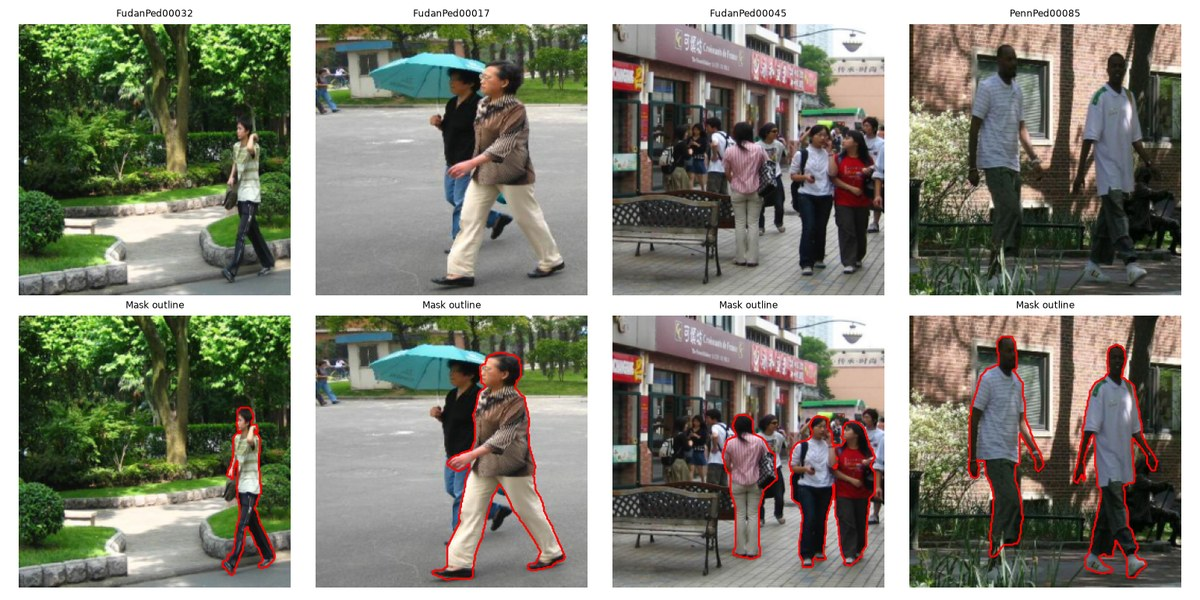
\includegraphics[width=\linewidth]{figures/pipeline_check.jpg}
    \caption{Preprocessing verification: image, mask, and green boundary alignment contour.}
    \label{fig:pipeline_check}
\end{minipage}
\hfill
\begin{minipage}{0.48\textwidth}
    \centering
    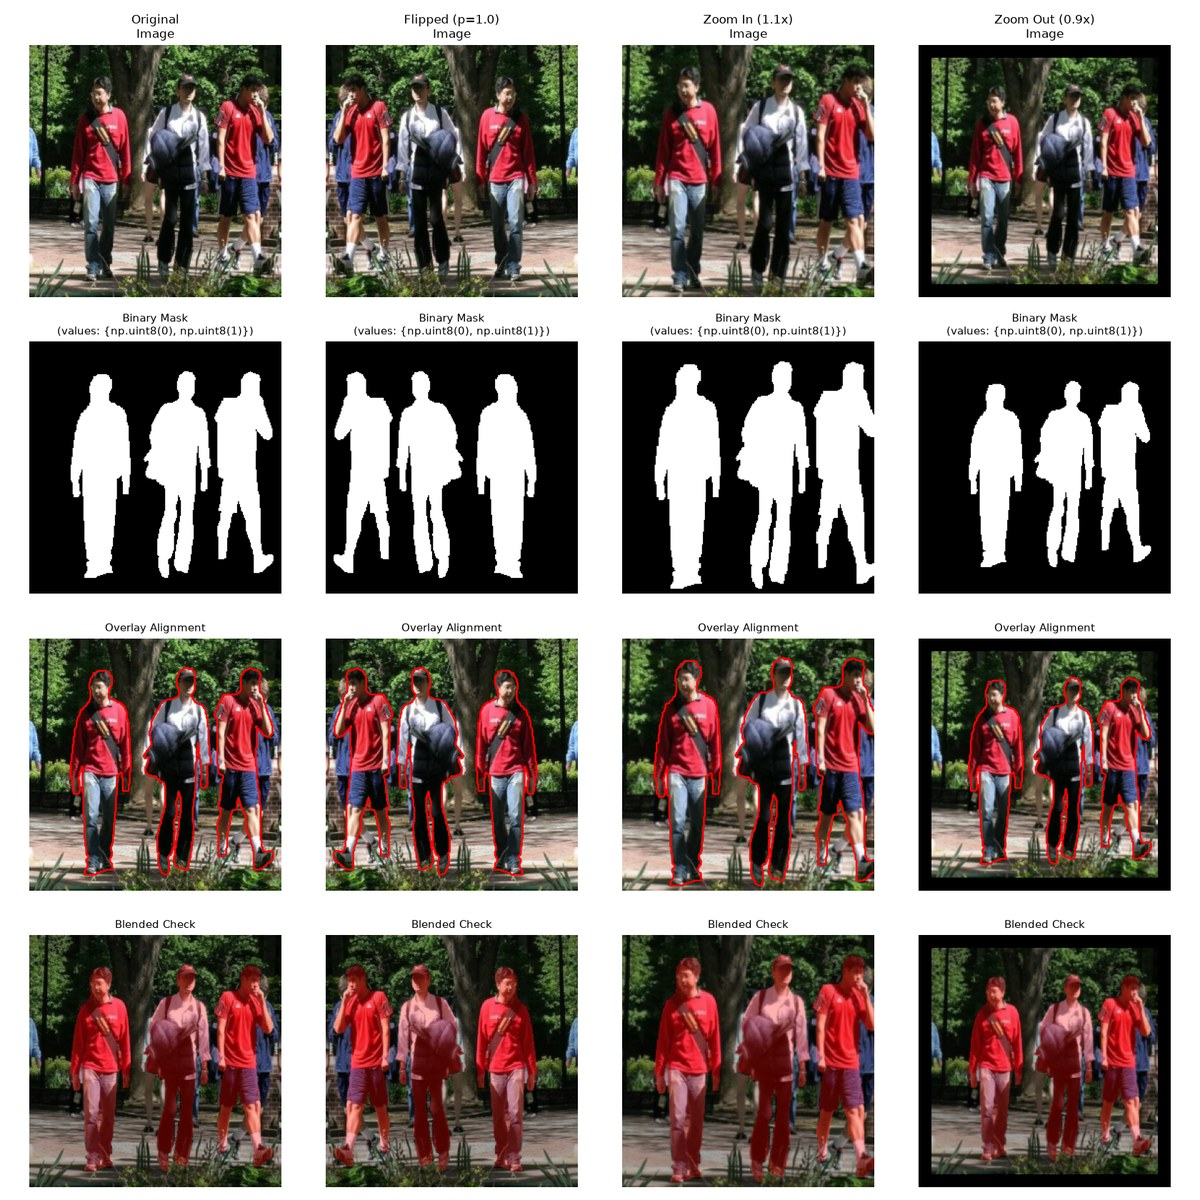
\includegraphics[width=\linewidth]{figures/augmentation_check.jpg}
    \caption{Synchronized augmentation (\texttt{flip\_zoom}): reflection and scale perturbation.}
    \label{fig:augmentation_check}
\end{minipage}
\end{figure}

\subsection{Synchronized Data Augmentation Pipeline}
To combat overfitting on the $118$ training images, we developed a synchronized geometric data augmentation engine (\texttt{flip\_zoom}):
\begin{enumerate}
    \item \textbf{Random Horizontal Flip ($p = 0.5$):} Mirrors both image and mask horizontally with probability $0.5$.
    \item \textbf{Random Multi-Scale Zoom ($s \in [0.9, 1.1]$):} Applies a uniform random scaling factor $s \sim \mathcal{U}(0.9, 1.1)$ followed by centered cropping or zero-padding back to $256 \times 256$.
\end{enumerate}
Augmentations are applied exclusively during training; validation and test sets remain strictly unaugmented.

\section{Exploratory Data Analysis (EDA)}
Prior to model training, statistical exploratory data analysis across all $170$ dataset samples revealed:
\begin{itemize}
    \item \textbf{Severe Class Imbalance:} Pedestrian pixels occupy only $23.2\%$ of the cumulative image surface area, while background pixels constitute $76.8\%$. On individual images, coverage ranges from $5.1\%$ to $43.8\%$.
    \item \textbf{Instance Density:} $58.2\%$ of images contain exactly two pedestrians, $24.7\%$ contain one pedestrian, and $17.1\%$ contain three or more pedestrians with frequent occlusions.
    \item \textbf{Spatial Distribution Bias:} Pedestrians are concentrated vertically within the central two-thirds of the horizontal frame, with zero pedestrian occurrence in the top $10\%$ of images.
\end{itemize}

\begin{figure}[htbp]
\centering
\begin{minipage}{0.45\textwidth}
    \centering
    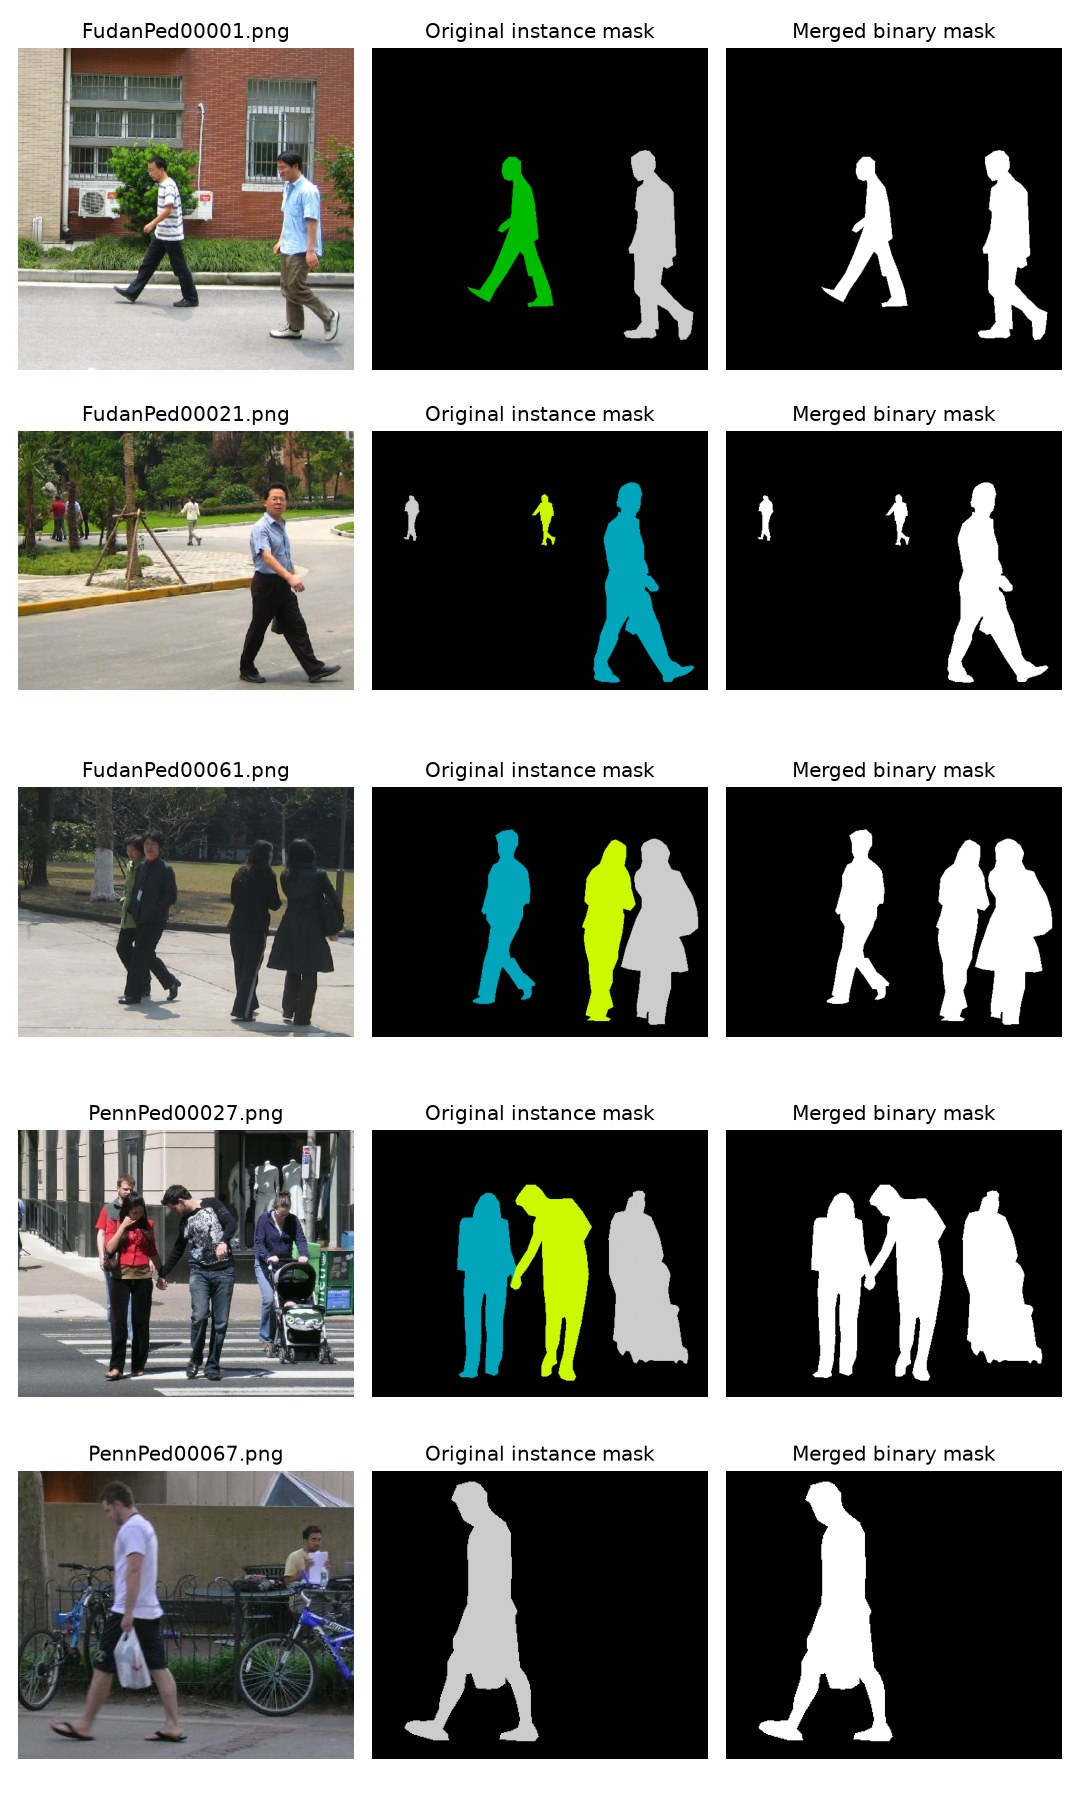
\includegraphics[width=\linewidth]{figures/dataset_check.jpg}
    \caption{EDA visual breakdown: raw image, multi-instance mask, and unified binary mask.}
    \label{fig:dataset_check}
\end{minipage}
\hfill
\begin{minipage}{0.51\textwidth}
    \centering
    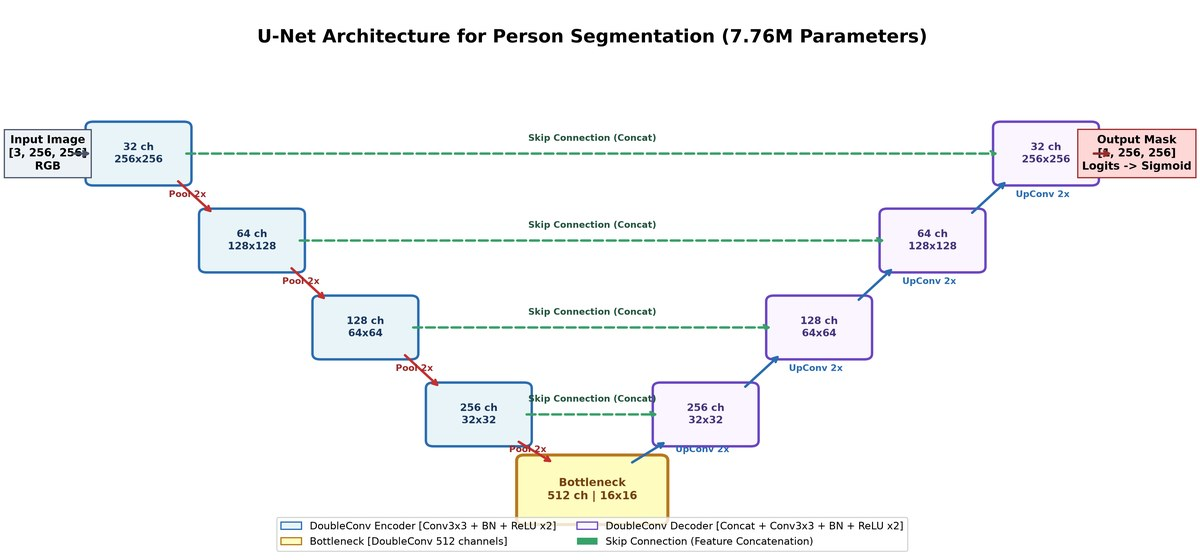
\includegraphics[width=\linewidth]{figures/unet_architecture.jpg}
    \caption{Proposed U-Net Architecture: 4 down/up stages with skip concatenation.}
    \label{fig:unet_arch}
\end{minipage}
\end{figure}

\section{Proposed U-Net Model Architecture}
To achieve high-fidelity person segmentation, we implemented a custom, modular U-Net \cite{ronneberger2015unet} architecture from scratch in PyTorch \cite{paszke2019pytorch} comprising four modular building blocks:

\subsubsection{1. Double Convolution Block ($\mathcal{F}_{\text{DoubleConv}}$)}
Each resolution level in both the encoder and decoder paths applies two consecutive $3 \times 3$ convolutions, each followed by Batch Normalization (BN) and ReLU activation:
\begin{align}
\mathbf{Z}^{(1)} &= \text{ReLU}\left(\text{BN}\left(\mathbf{W}^{(1)} * \mathbf{X} + \mathbf{b}^{(1)}\right)\right), \\
\mathbf{Z}^{(2)} &= \text{ReLU}\left(\text{BN}\left(\mathbf{W}^{(2)} * \mathbf{Z}^{(1)} + \mathbf{b}^{(2)}\right)\right),
\end{align}
with kernel size $3 \times 3$, stride $1$, and padding $1$, strictly preserving intermediate spatial dimensions.

\subsubsection{2. Contracting (Downsampling) Block ($\mathcal{F}_{\text{Down}}$)}
Spatial dimensions are halved using a $2 \times 2$ Max Pooling operation with stride $2$, followed by a Double Convolution block:
\begin{equation}
\mathbf{X}_{l} = \mathcal{F}_{\text{DoubleConv}}\left(\text{MaxPool}_{2\times 2}(\mathbf{X}_{l-1})\right), \quad l \in \{1, 2, 3, 4\}.
\end{equation}

\subsubsection{3. Expanding (Upsampling) Block ($\mathcal{F}_{\text{Up}}$)}
In the decoder path, spatial feature maps are upsampled using a $2 \times 2$ Transposed Convolution (stride $2$) and concatenated with the skip feature map $\mathbf{S}_l$ from the encoder:
\begin{equation}
\mathbf{U}_l = \text{ConvTranspose2d}_{2\times 2}(\mathbf{X}_{l}), \quad \mathbf{X}_{l-1}^{\text{dec}} = \mathcal{F}_{\text{DoubleConv}}\left(\left[\mathbf{U}_l \,\|\, \mathbf{S}_l\right]\right).
\end{equation}

\subsubsection{4. Output Projection Layer ($\mathcal{F}_{\text{Out}}$)}
The final feature map at $256 \times 256$ is projected to a single-channel logit map via a $1 \times 1$ convolution:
\begin{equation}
\hat{\mathbf{Z}} = \mathbf{W}_{\text{out}} * \mathbf{X}_{0}^{\text{dec}} + \mathbf{b}_{\text{out}} \in \mathbb{R}^{B \times 1 \times 256 \times 256}.
\end{equation}

Table~\ref{tab:unet_specs} outlines the complete tensor dimensions and parameter distribution across the network for our baseline capacity ($C = 32$ base channels).

\begin{table}[htbp]
\centering
\small
\caption{Layer-by-Layer Architectural Specifications of the Proposed U-Net ($C=32$)}
\label{tab:unet_specs}
\begin{tabular}{llccr}
\toprule
\textbf{Stage} & \textbf{Module Name} & \textbf{Input Resolution} & \textbf{Output Shape} & \textbf{Parameters} \\
\midrule
Input & Input Image & $256 \times 256 \times 3$ & $[B, 3, 256, 256]$ & 0 \\
Encoder 1 & DoubleConv 1 & $256 \times 256 \times 3$ & $[B, 32, 256, 256]$ & 10,208 \\
Encoder 2 & Down 1 & $[B, 32, 256, 256]$ & $[B, 64, 128, 128]$ & 55,616 \\
Encoder 3 & Down 2 & $[B, 64, 128, 128]$ & $[B, 128, 64, 64]$ & 221,824 \\
Encoder 4 & Down 3 & $[B, 128, 64, 64]$ & $[B, 256, 32, 32]$ & 886,016 \\
Bottleneck & Down 4 & $[B, 256, 32, 32]$ & $[B, 512, 16, 16]$ & 3,541,504 \\
Decoder 1 & Up 1 & $[B, 512, 16, 16]$ & $[B, 256, 32, 32]$ & 1,770,240 \\
Decoder 2 & Up 2 & $[B, 256, 32, 32]$ & $[B, 128, 64, 64]$ & 442,752 \\
Decoder 3 & Up 3 & $[B, 128, 64, 64]$ & $[B, 64, 128, 128]$ & 110,784 \\
Decoder 4 & Up 4 & $[B, 64, 128, 128]$ & $[B, 32, 256, 256]$ & 27,744 \\
Output & OutConv ($1\times 1$) & $[B, 32, 256, 256]$ & $[B, 1, 256, 256]$ & 33 \\
\midrule
\textbf{Total} & \textbf{U-Net ($C=32$)} & & & \textbf{7,766,721} \\
\bottomrule
\end{tabular}
\end{table}

\section{Hybrid Loss Function Formulation}
We formulate a composite objective combining Binary Cross-Entropy with logits and smooth soft Dice Loss:
\begin{equation}
\mathcal{L}_{\text{total}}(\hat{\mathbf{z}}, \mathbf{y}) = \alpha \cdot \mathcal{L}_{\text{BCE}}(\hat{\mathbf{z}}, \mathbf{y}) + \beta \cdot \mathcal{L}_{\text{Dice}}(\hat{\mathbf{z}}, \mathbf{y}),
\end{equation}
where $\mathcal{L}_{\text{BCE}}(\hat{\mathbf{z}}, \mathbf{y}) = \frac{1}{N} \sum_{i=1}^{N} [ \max(\hat{z}_i, 0) - \hat{z}_i y_i + \log(1 + e^{-|\hat{z}_i|}) ]$ stabilizes pixel-wise gradient flow, and $\mathcal{L}_{\text{Dice}}(\hat{\mathbf{z}}, \mathbf{y}) = 1 - \frac{2 \sum_{i=1}^N p_i y_i + 1.0}{\sum_{i=1}^N p_i + \sum_{i=1}^N y_i + 1.0}$ directly maximizes area overlap.

\section{Optimization Algorithm and Experimental Setup}
Algorithm~\ref{alg:training_pipeline} outlines the complete training, validation, and early stopping pipeline.

\begin{algorithm}[htbp]
\caption{End-to-End U-Net Training and Validation Pipeline with Early Stopping}
\label{alg:training_pipeline}
\begin{algorithmic}[1]
\Require $\mathcal{D}_{\text{train}}$, $\mathcal{D}_{\text{val}}$, Model parameters $\Theta$, Learning rate $\eta=5\times 10^{-4}$, Batch size $B=8$, Max epochs $E_{\max}=100$, Patience $P=20$, Loss weights $(\alpha=1.5, \beta=0.5)$, Threshold $\tau = 0.5$.
\Ensure Optimal model checkpoint $\Theta^*$.
\State Initialize $\Theta$ using Kaiming normal; initialize Adam ($\beta_1=0.9, \beta_2=0.999$), $\text{IoU}_{\text{best}} \gets 0.0$.
\For{epoch $e = 1$ to $E_{\max}$}
    \State $\text{Model}.\text{train}()$; Forward batches with flip \& zoom; Compute $\mathcal{L} = 1.5\mathcal{L}_{\text{BCE}} + 0.5\mathcal{L}_{\text{Dice}}$; $\text{Opt}.\text{step}()$.
    \State $\text{Model}.\text{eval}()$; \textbf{with } $\text{torch}.\text{no\_grad}()$: Compute $\text{TP}_{\text{val}}, \text{FP}_{\text{val}}, \text{FN}_{\text{val}}, \text{TN}_{\text{val}}$ on validation split.
    \State $\text{IoU}_{\text{val}} \gets \frac{\text{TP}_{\text{val}}}{\text{TP}_{\text{val}} + \text{FP}_{\text{val}} + \text{FN}_{\text{val}}}$; $\text{Scheduler}.\text{step}(\text{IoU}_{\text{val}})$.
    \If{$\text{IoU}_{\text{val}} > \text{IoU}_{\text{best}}$}
        \State $\text{IoU}_{\text{best}} \gets \text{IoU}_{\text{val}}$; $\Theta^* \gets \Theta$; Save checkpoint to \texttt{"checkpoint\_best.pt"}; $\text{counter} \gets 0$.
    \Else
        \State $\text{counter} \gets \text{counter} + 1$; \textbf{if } $\text{counter} \ge P$ \textbf{then break} (Early Stopping).
    \EndIf
\EndFor
\State \Return Optimal checkpoint $\Theta^*$.
\end{algorithmic}
\end{algorithm}

% ------------------------------------------------------------------------------
% CHAPTER 4: RESULTS AND DISCUSSION
% ------------------------------------------------------------------------------
\chapter{Results and Discussion}
\label{chap:results_discussion}

\section{Performance Evaluation Metrics}
Predictions are thresholded at $\tau = 0.5$: $\hat{y}_i = \mathbb{I}(\sigma(\hat{z}_i) \ge 0.5)$. Performance is evaluated using True Positives (TP), False Positives (FP), False Negatives (FN), and True Negatives (TN):
\begin{equation}
\text{Precision} = \frac{\text{TP}}{\text{TP} + \text{FP}}, \quad
\text{Recall} = \frac{\text{TP}}{\text{TP} + \text{FN}}, \quad
\text{F1} = \frac{2\cdot \text{TP}}{2\cdot \text{TP} + \text{FP} + \text{FN}}, \quad
\text{IoU} = \frac{\text{TP}}{\text{TP} + \text{FP} + \text{FN}}.
\end{equation}
Metrics are reported both as \textbf{Global Pixel-Level} aggregates and \textbf{Mean Per-Image} averages ($\pm$ standard deviation).

\section{Experimental Results Across Optimization Phases}
Table~\ref{tab:cross_phase_comparison} documents the cross-phase progression evaluated on the untouched $25$-image validation set.

\begin{table}[htbp]
\centering
\small
\caption{Cross-Phase Experimental Comparison on the Validation Set ($25$ Images)}
\label{tab:cross_phase_comparison}
\begin{tabular}{lccccccr}
\toprule
\textbf{Experimental Configuration} & \textbf{Aug.} & \textbf{LR} & \textbf{Weights ($\alpha / \beta$)} & \textbf{Epoch} & \textbf{Val IoU} & \textbf{Val F1} & \textbf{Time} \\
\midrule
Phase 5: Baseline (No Aug) & None & $10^{-3}$ & $1.0 / 1.0$ & 32 & 0.7447 & 0.8536 & 5.7m \\
Phase 6: Geometric Augmentation & Flip+Zoom & $10^{-3}$ & $1.0 / 1.0$ & 73 & 0.7635 & 0.8659 & 10.9m \\
Phase 7: Learning Rate ($10^{-4}$) & Flip+Zoom & $10^{-4}$ & $1.0 / 1.0$ & 27 & 0.7186 & 0.8363 & 5.8m \\
Phase 7: Learning Rate ($5\times 10^{-4}$) & Flip+Zoom & $5\times 10^{-4}$ & $1.0 / 1.0$ & 75 & 0.7669 & 0.8681 & 11.3m \\
Phase 8: Loss Weights ($0.5 / 1.5$) & Flip+Zoom & $5\times 10^{-4}$ & $0.5 / 1.5$ & 29 & 0.7685 & 0.8691 & 5.4m \\
\textbf{Phase 8: Loss Weights ($1.5 / 0.5$)$^*$} & \textbf{Flip+Zoom} & $\mathbf{5\times 10^{-4}}$ & $\mathbf{1.5 / 0.5}$ & \textbf{57} & \textbf{0.7739} & \textbf{0.8725} & \textbf{9.6m} \\
Phase 9: Capacity ($C=16$, $1.94$M) & Flip+Zoom & $5\times 10^{-4}$ & $1.5 / 0.5$ & 33 & 0.7414 & 0.8515 & 2.2m \\
Phase 9: Capacity ($C=48$, $17.46$M) & Flip+Zoom & $5\times 10^{-4}$ & $1.5 / 0.5$ & 56 & 0.7627 & 0.8653 & 20.1m \\
\bottomrule
\multicolumn{8}{l}{\footnotesize $^*$Selected as the optimal model configuration for final Phase 10 test evaluation.}
\end{tabular}
\end{table}

\subsection{Ablation Findings}
\begin{itemize}
    \item \textbf{Data Augmentation (Phase 6):} Synchronized flipping and zoom delayed early stopping from epoch 32 to 73, elevating validation IoU from $0.7447$ to $0.7635$ ($+2.53\%$ relative gain).
    \item \textbf{Learning Rate (Phase 7):} $\eta = 5\times 10^{-4}$ achieved peak convergence (IoU $0.7669$), outperforming lower ($10^{-4}$, IoU $0.7186$) and higher ($10^{-3}$, IoU $0.7635$) rates.
    \item \textbf{Loss Weights (Phase 8):} Asymmetric weighting ($\alpha=1.5, \beta=0.5$) yielded the highest validation score across all experiments: $\mathbf{0.7739}$ IoU and $\mathbf{0.8725}$ F1. Emphasizing BCE provides strong gradient signals that suppress false positive background clutter.
    \item \textbf{Model Capacity (Phase 9):} $C=32$ base channels ($7.76$M parameters) represents the optimal capacity. Reducing to $C=16$ ($1.94$M) caused underfitting (IoU $0.7414$), while scaling to $C=48$ ($17.46$M) resulted in overfitting (IoU $0.7627$) and redundant compute.
\end{itemize}

\section{Final Test Set Evaluation (Phase 10)}
The selected optimal model (\texttt{checkpoints/loss\_15\_05\_best.pt}) was evaluated exactly once on the pristine test split of $27$ urban images ($54$ pedestrian instances). Table~\ref{tab:test_metrics} documents the final test results.

\begin{table}[htbp]
\centering
\small
\caption{Comprehensive Final Test Set Performance Metrics ($27$ Unseen Images)}
\label{tab:test_metrics}
\begin{tabular}{lcc}
\toprule
\textbf{Evaluation Metric} & \textbf{Global Pixel-Level} & \textbf{Mean Per-Image ($\pm \text{Std}$)} \\
\midrule
Intersection-over-Union (IoU) & \textbf{0.7483} & \textbf{0.7616} $\pm$ \textbf{0.1339} \\
F1-Score (Dice Coefficient) & \textbf{0.8560} & \textbf{0.8573} $\pm$ \textbf{0.1084} \\
Precision & \textbf{0.8214} & \textbf{0.8305} $\pm$ \textbf{0.1075} \\
Recall (Sensitivity) & \textbf{0.8936} & \textbf{0.9063} $\pm$ \textbf{0.0782} \\
\midrule
Test Losses & \multicolumn{2}{c}{BCE: $0.1456$, Dice: $0.2239$, Combined ($\alpha=1.5, \beta=0.5$): $0.3304$} \\
Cumulative Pixel Counts & \multicolumn{2}{c}{TP: $250,188$ | FP: $54,391$ | FN: $29,776$ | TN: $1,435,117$} \\
\bottomrule
\end{tabular}
\end{table}

\begin{figure}[htbp]
\centering
\begin{minipage}{0.54\textwidth}
    \centering
    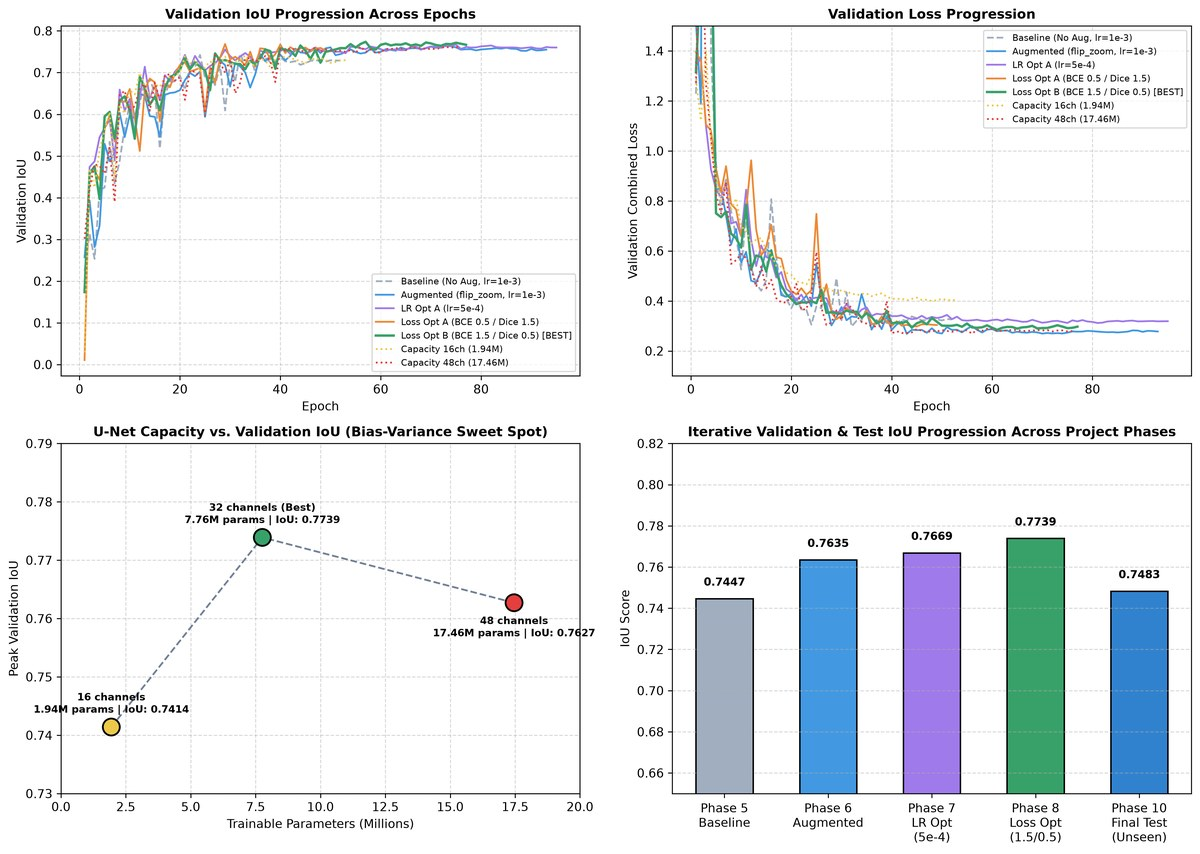
\includegraphics[width=\linewidth]{figures/training_progression.jpg}
    \caption{Multi-panel training dynamics: loss decay, IoU trajectories, and capacity curve.}
    \label{fig:training_progression}
\end{minipage}
\hfill
\begin{minipage}{0.42\textwidth}
    \centering
    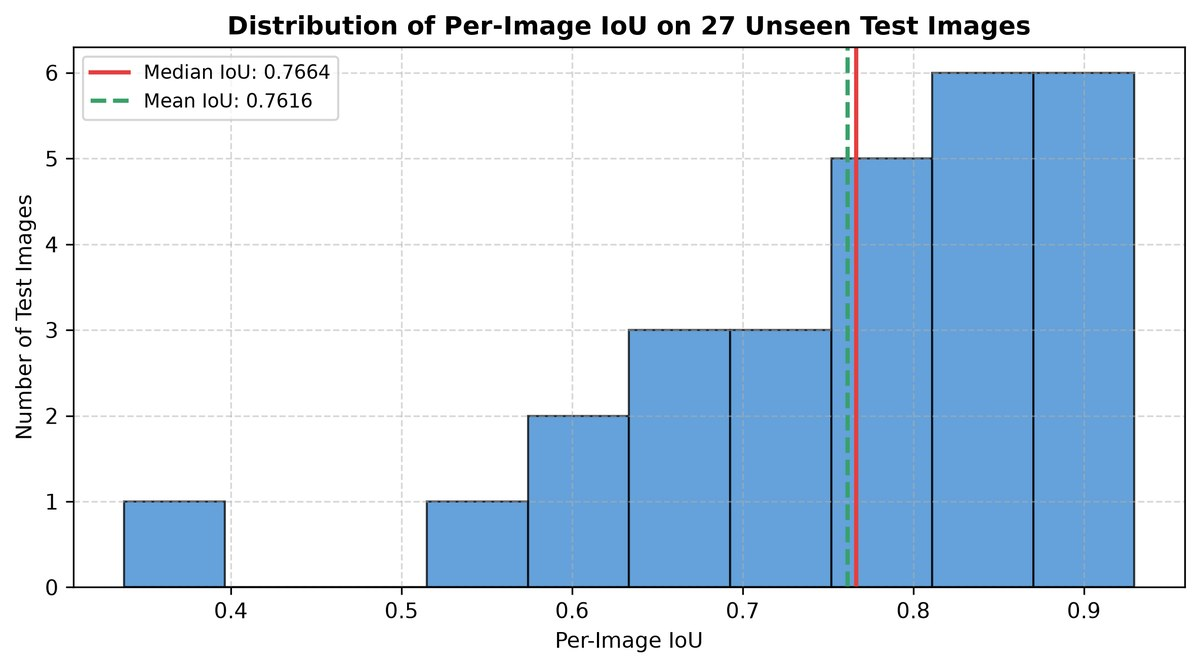
\includegraphics[width=\linewidth]{figures/test_iou_distribution.jpg}
    \caption{Per-image test IoU distribution histogram (median: $0.7664$, mean: $0.7616$).}
    \label{fig:test_distribution}
\end{minipage}
\end{figure}

\section{Qualitative Error and Failure Mode Analysis}
\begin{figure}[htbp]
\centering
\begin{minipage}{0.32\textwidth}
    \centering
    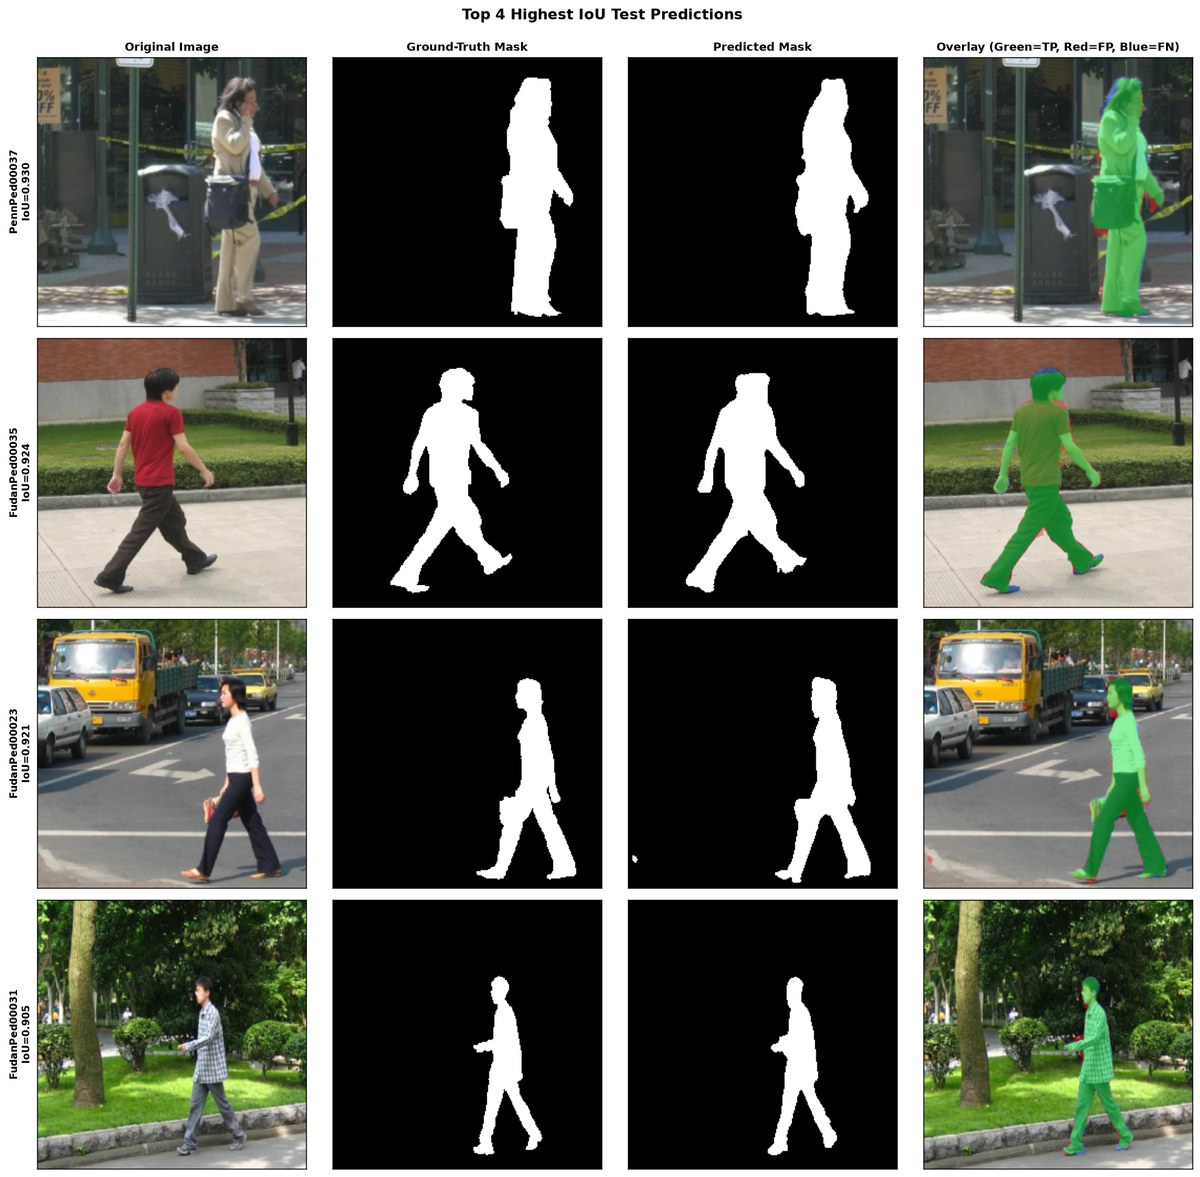
\includegraphics[width=\linewidth]{figures/grid_top_4.jpg}
    \caption{Top predictions (IoU $> 0.88$).}
    \label{fig:grid_top}
\end{minipage}
\hfill
\begin{minipage}{0.32\textwidth}
    \centering
    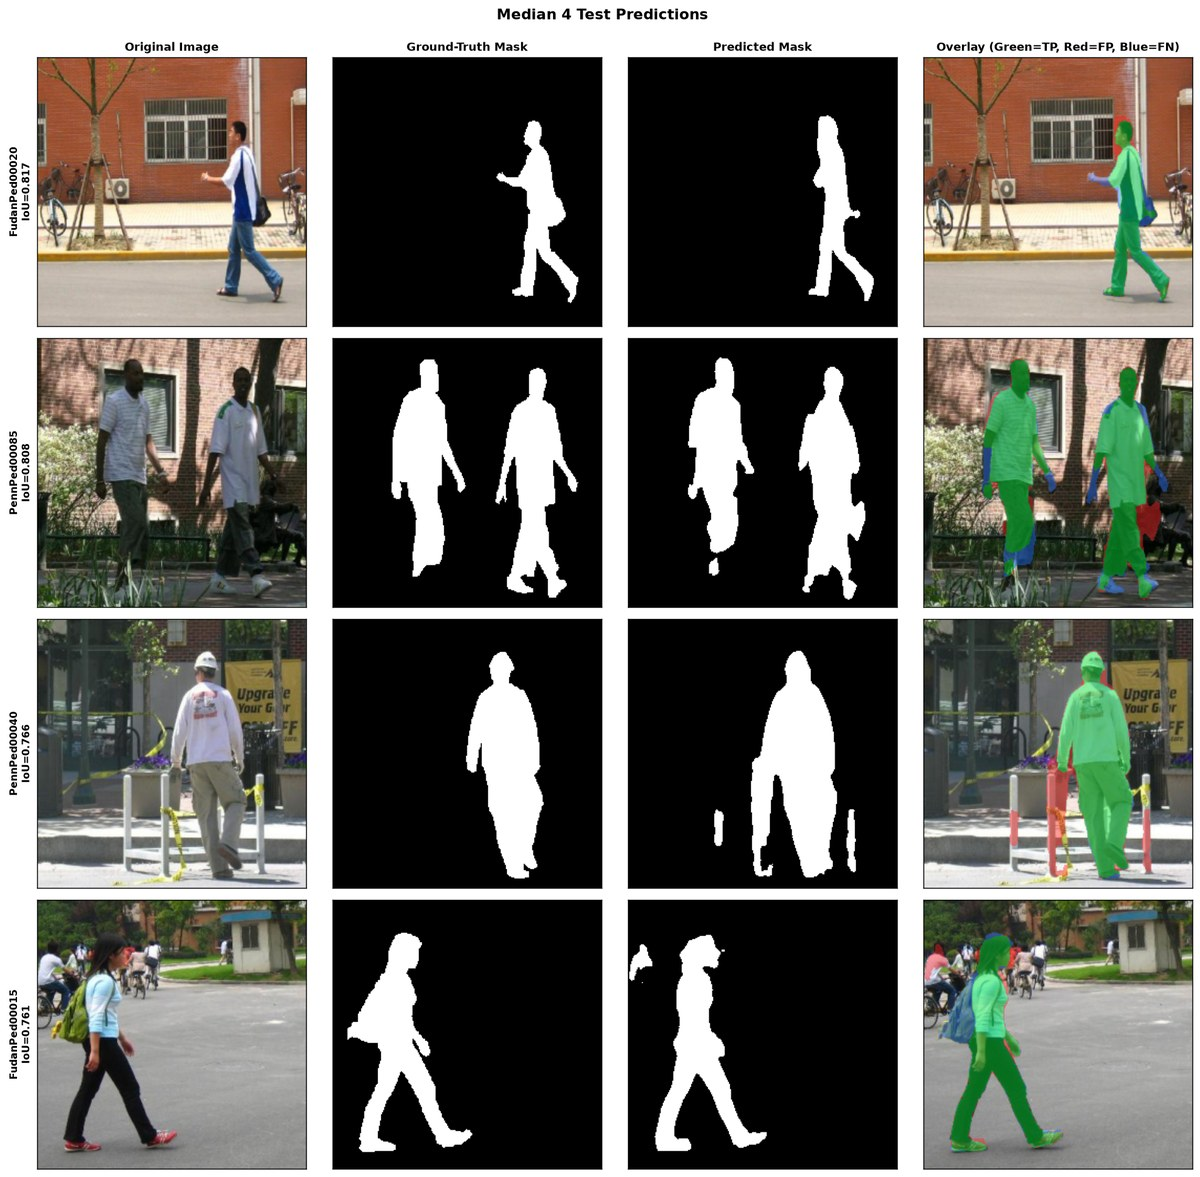
\includegraphics[width=\linewidth]{figures/grid_median_4.jpg}
    \caption{Median predictions (0.75--0.77).}
    \label{fig:grid_median}
\end{minipage}
\hfill
\begin{minipage}{0.32\textwidth}
    \centering
    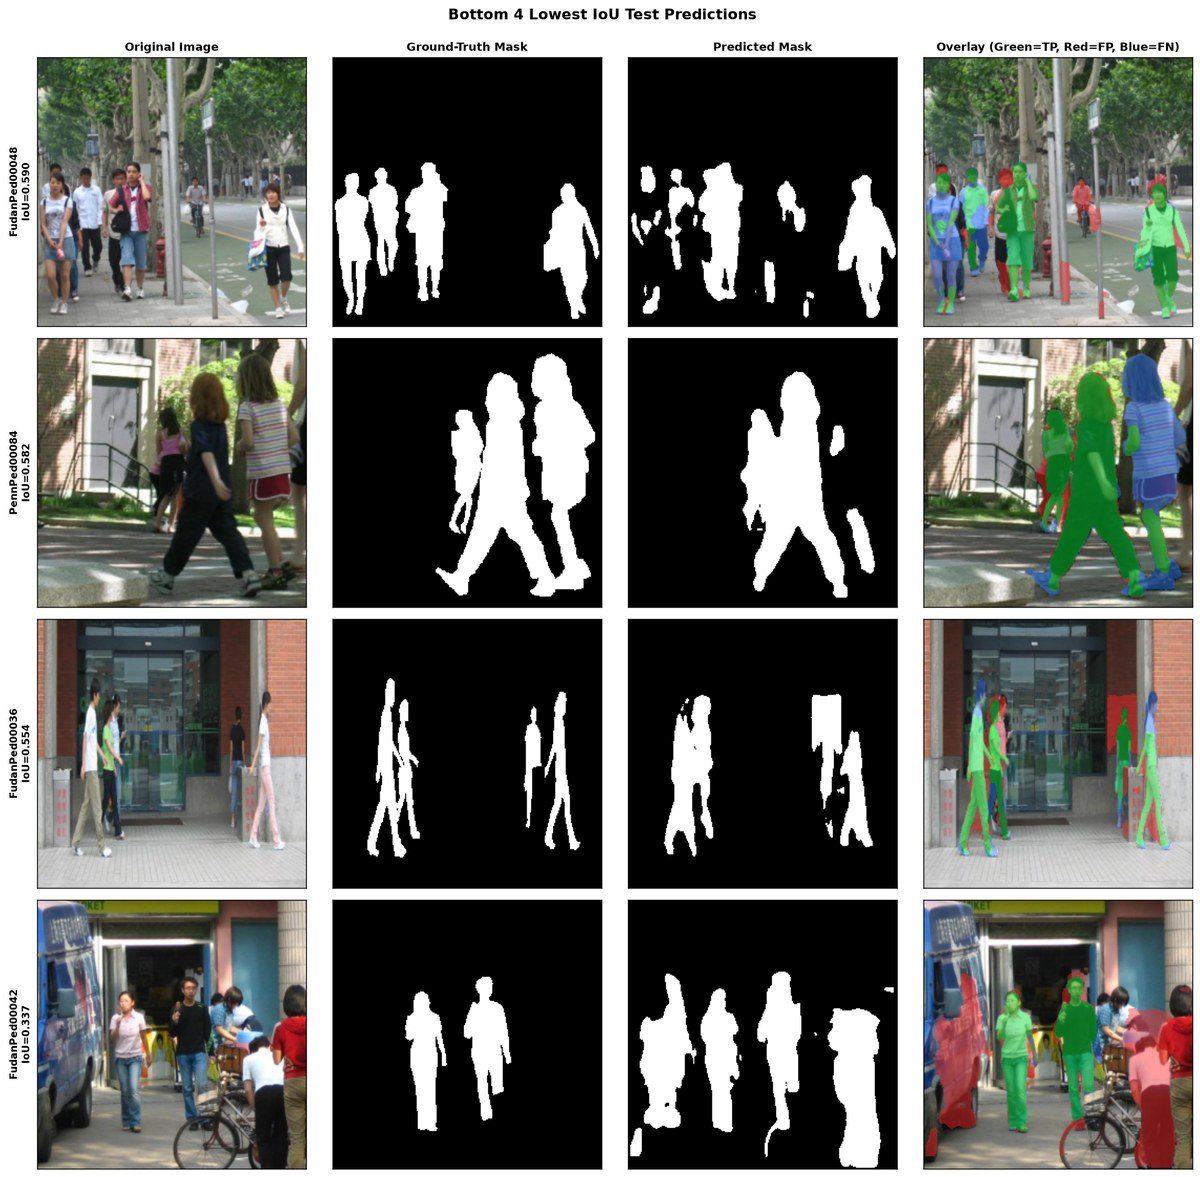
\includegraphics[width=\linewidth]{figures/grid_worst_4.jpg}
    \caption{Challenging test samples.}
    \label{fig:grid_worst}
\end{minipage}
\end{figure}

\subsection{Ground-Truth Annotation Noise Discovery}
A crucial empirical discovery emerged upon examining the lowest-scoring test sample \texttt{FudanPed00042} (IoU: $0.3373$, Figure~\ref{fig:grid_worst}):
\begin{itemize}
    \item The original Penn-Fudan ground-truth annotated only the two prominent foreground pedestrians.
    \item However, the scene contains a third pedestrian in a red shirt and a fourth person riding a bicycle in the mid-ground.
    \item The trained U-Net correctly segmented both the red-shirt pedestrian and the cyclist.
    \item Because these individuals were omitted from the official ground-truth mask, all corresponding pixels were registered as False Positives, depressing computed precision to $0.3438$ and IoU to $0.3373$.
\end{itemize}
This demonstrates that the model's true visual segmentation capacity is even higher than aggregate benchmark metrics indicate.

% ------------------------------------------------------------------------------
% CHAPTER 5: CONCLUSION AND FUTURE SCOPE
% ------------------------------------------------------------------------------
\chapter{Conclusion and Future Scope}
\label{chap:conclusion}

\section{Key Findings}
This college project implemented and validated an end-to-end binary person segmentation framework on the Penn-Fudan dataset using a from-scratch U-Net architecture. Key empirical findings include:
\begin{enumerate}
    \item Synchronized geometric data augmentation (\texttt{flip\_zoom}) successfully regularized small-sample training ($118$ images), extending convergence from epoch 32 to 73 and providing a $+2.53\%$ relative IoU improvement.
    \item Optimization exploration showed that learning rate $\eta = 5\times 10^{-4}$ with Adam and ReduceLROnPlateau provided the most stable gradient updates.
    \item Asymmetric hybrid loss weighting ($\alpha=1.5, \beta=0.5$) outperformed standard equal weighting, delivering our peak validation IoU of $\mathbf{0.7739}$ and F1 of $\mathbf{0.8725}$.
    \item Model capacity scaling identified $C=32$ base channels ($7.76$M parameters) as the optimal capacity boundary, striking the ideal bias-variance trade-off.
    \item On $27$ untouched test scenes, the model demonstrated robust generalization: $\mathbf{0.7483}$ Global IoU, $\mathbf{0.8560}$ Global F1, and $\mathbf{0.8936}$ Recall, with outliers driven by dataset annotation omissions rather than model failure.
\end{enumerate}

\section{Limitations and Future Scope}
\textbf{Limitations:} Fixed $256 \times 256$ input resolution introduces aspect ratio distortions on wide images; binary formulation collapses overlapping instances into single silhouettes; and training is constrained to daylight campus scenes.

\noindent\textbf{Future Directions:} Future work can incorporate multi-task instance embedding heads for individual pedestrian tracking, spatial and channel attention mechanisms (Attention U-Net / TransUNet), multi-scale feature pyramids for high-resolution video streams, and model quantization (INT8) for real-time embedded edge deployment.

% ==============================================================================
% END MATTER
% ==============================================================================

\begin{thebibliography}{99}
\addcontentsline{toc}{chapter}{References}
\bibitem{ronneberger2015unet} O.~Ronneberger, P.~Fischer, and T.~Brox, ``U-Net: Convolutional Networks for Biomedical Image Segmentation,'' in \emph{MICCAI}, vol. 9351, pp. 234--241, 2015.
\bibitem{long2015fcn} J.~Long, E.~Shelhamer, and T.~Darrell, ``Fully Convolutional Networks for Semantic Segmentation,'' in \emph{CVPR}, pp. 3431--3440, 2015.
\bibitem{chen2017deeplab} L.-C. Chen et~al., ``DeepLab: Semantic Image Segmentation with Deep Convolutional Nets, Atrous Convolution, and Fully Connected CRFs,'' \emph{IEEE TPAMI}, vol.~40, no.~4, pp. 834--848, 2017.
\bibitem{he2017maskrcnn} K.~He, G.~Gkioxari, P.~Doll{\'a}r, and R.~Girshick, ``Mask R-CNN,'' in \emph{ICCV}, pp. 2961--2969, 2017.
\bibitem{milletari2016vnet} F.~Milletari, N.~Navab, and S.-A. Ahmadi, ``V-Net: Fully Convolutional Networks for Volumetric Medical Image Segmentation,'' in \emph{3DV}, pp. 565--571, 2016.
\bibitem{lin2017focal} T.-Y. Lin et~al., ``Focal Loss for Dense Object Detection,'' in \emph{ICCV}, pp. 2980--2988, 2017.
\bibitem{wang2007pennfudan} L.~Wang, J.~Shi, G.~Song, and I.-f. Shen, ``Object Detection Combining Recognition and Segmentation,'' \emph{IEEE TPAMI}, vol.~30, no.~7, pp. 1270--1285, 2008.
\bibitem{kingma2014adam} D.~P. Kingma and J.~Ba, ``Adam: A Method for Stochastic Optimization,'' \emph{arXiv:1412.6980}, 2014.
\bibitem{dalal2005hog} N.~Dalal and B.~Triggs, ``Histograms of Oriented Gradients for Human Detection,'' in \emph{CVPR}, vol.~1, pp. 886--893, 2005.
\bibitem{felzenszwalb2009dpm} P.~F. Felzenszwalb et~al., ``Object Detection with Discriminatively Trained Part-Based Models,'' \emph{IEEE TPAMI}, vol.~32, no.~9, pp. 1627--1645, 2009.
\bibitem{badrinarayanan2017segnet} V.~Badrinarayanan, A.~Kendall, and R.~Cipolla, ``SegNet: A Deep Convolutional Encoder-Decoder Architecture for Image Segmentation,'' \emph{IEEE TPAMI}, vol.~39, no.~12, pp. 2481--2495, 2017.
\bibitem{jadon2020survey} S.~Jadon, ``A Survey of Loss Functions for Semantic Segmentation,'' in \emph{IEEE CIBCB}, pp. 1--7, 2020.
\bibitem{paszke2019pytorch} A.~Paszke et~al., ``PyTorch: An Imperative Style, High-Performance Deep Learning Library,'' in \emph{NeurIPS}, vol.~32, pp. 8024--8035, 2019.
\bibitem{shorten2019survey} C.~Shorten and T.~M. Khoshgoftaar, ``A Survey on Image Data Augmentation for Deep Learning,'' \emph{Journal of Big Data}, vol.~6, no.~1, pp. 1--48, 2019.
\bibitem{sudre2017generalised} C.~H. Sudre et~al., ``Generalised Dice Overlap as a Deep Learning Loss Function for Highly Unbalanced Segmentations,'' in \emph{DLMIA}, pp. 240--248, 2017.
\end{thebibliography}

\chapter*{Appendix: Detailed Per-Image Test Evaluation}
\addcontentsline{toc}{chapter}{Appendix}
\label{chap:appendix}

Table~\ref{tab:appendix_per_image} details the complete, image-by-image quantitative performance metrics computed during Phase 10 across all $27$ test images from the Penn-Fudan benchmark using the selected optimal model (\texttt{checkpoints/loss\_15\_05\_best.pt}).

\begin{table}[htbp]
\centering
\scriptsize
\caption{Detailed Per-Image Test Evaluation Results across the 27 Test Images}
\label{tab:appendix_per_image}
\begin{tabular}{lccccccrr}
\toprule
\textbf{Image Name} & \textbf{IoU} & \textbf{F1-Score} & \textbf{Precision} & \textbf{Recall} & \textbf{TP} & \textbf{FP} & \textbf{FN} & \textbf{TN} \\
\midrule
PennPed00037 & 0.9295 & 0.9635 & 0.9634 & 0.9635 & 9,090 & 345 & 344 & 55,757 \\
FudanPed00035 & 0.9243 & 0.9607 & 0.9522 & 0.9693 & 9,120 & 458 & 289 & 55,669 \\
FudanPed00023 & 0.9207 & 0.9587 & 0.9453 & 0.9726 & 6,063 & 351 & 171 & 58,951 \\
FudanPed00031 & 0.9052 & 0.9502 & 0.9422 & 0.9585 & 3,877 & 238 & 168 & 61,253 \\
FudanPed00050 & 0.9023 & 0.9487 & 0.9315 & 0.9664 & 5,524 & 406 & 192 & 59,414 \\
FudanPed00059 & 0.8705 & 0.9307 & 0.8827 & 0.9843 & 14,360 & 1,908 & 229 & 49,039 \\
PennPed00029 & 0.8700 & 0.9305 & 0.9416 & 0.9196 & 14,087 & 873 & 1,232 & 49,344 \\
PennPed00066 & 0.8546 & 0.9216 & 0.8819 & 0.9649 & 15,217 & 2,037 & 553 & 47,729 \\
FudanPed00065 & 0.8382 & 0.9120 & 0.9169 & 0.9071 & 19,402 & 1,758 & 1,986 & 42,390 \\
PennPed00024 & 0.8304 & 0.9074 & 0.8983 & 0.9166 & 6,729 & 762 & 612 & 57,433 \\
PennPed00004 & 0.8185 & 0.9002 & 0.9214 & 0.8800 & 14,349 & 1,224 & 1,957 & 48,006 \\
FudanPed00020 & 0.8166 & 0.8990 & 0.9249 & 0.8746 & 3,842 & 312 & 551 & 60,831 \\
PennPed00085 & 0.8076 & 0.8935 & 0.9098 & 0.8779 & 13,115 & 1,301 & 1,824 & 49,296 \\
PennPed00040 & 0.7664 & 0.8678 & 0.7725 & 0.9898 & 9,257 & 2,726 & 95 & 53,458 \\
FudanPed00015 & 0.7612 & 0.8644 & 0.8990 & 0.8324 & 7,029 & 790 & 1,415 & 56,302 \\
PennPed00068 & 0.7604 & 0.8639 & 0.8940 & 0.8357 & 12,534 & 1,486 & 2,464 & 49,052 \\
FudanPed00045 & 0.7533 & 0.8593 & 0.8379 & 0.8818 & 10,438 & 2,019 & 1,399 & 51,680 \\
PennPed00067 & 0.7221 & 0.8386 & 0.7668 & 0.9252 & 7,732 & 2,351 & 625 & 54,828 \\
FudanPed00007 & 0.7010 & 0.8242 & 0.7153 & 0.9723 & 10,310 & 4,103 & 294 & 50,829 \\
FudanPed00032 & 0.6947 & 0.8199 & 0.7152 & 0.9604 & 3,054 & 1,216 & 126 & 61,140 \\
PennPed00063 & 0.6920 & 0.8180 & 0.7309 & 0.9285 & 8,497 & 3,128 & 654 & 53,257 \\
FudanPed00037 & 0.6870 & 0.8145 & 0.7177 & 0.9414 & 6,010 & 2,364 & 374 & 56,788 \\
FudanPed00017 & 0.6731 & 0.8046 & 0.6939 & 0.9573 & 10,213 & 4,505 & 456 & 50,362 \\
FudanPed00048 & 0.5899 & 0.7421 & 0.7711 & 0.7151 & 8,015 & 2,379 & 3,193 & 51,949 \\
PennPed00084 & 0.5823 & 0.7360 & 0.9185 & 0.6141 & 11,246 & 998 & 7,068 & 46,224 \\
FudanPed00036 & 0.5544 & 0.7133 & 0.6353 & 0.8133 & 5,089 & 2,922 & 1,168 & 56,357 \\
FudanPed00042 & 0.3373 & 0.5044 & 0.3438 & 0.9467 & 5,989 & 11,431 & 337 & 47,779 \\
\midrule
\textbf{Mean ($\pm\text{Std}$)} & \textbf{0.7616} & \textbf{0.8573} & \textbf{0.8305} & \textbf{0.9063} & \textbf{9,266} & \textbf{2,014} & \textbf{1,103} & \textbf{53,152} \\
\textbf{Global Sum} & \textbf{0.7483} & \textbf{0.8560} & \textbf{0.8214} & \textbf{0.8936} & \textbf{250,188} & \textbf{54,391} & \textbf{29,776} & \textbf{1,435,117} \\
\bottomrule
\end{tabular}
\end{table}

\end{document}
